%BEGIN TICKET 24
\begin{statement}
    $f$ --- периодическая функция с периодом  $T$. Тогда неважно, по какому периоду интегрировать$\Rightarrow$ $\int\limits_a^{a+T} f = \int\limits_b^{b+T}f$ 
\end{statement}
\begin{proof}
    см. картинку:\\
    \begin{figure}[h!]
        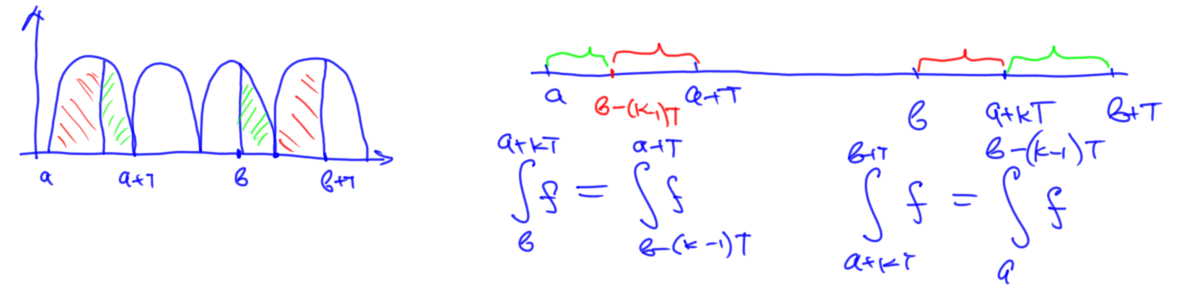
\includegraphics[scale=0.6]{abels_consequence}
    \end{figure}
    
    $\int\limits_b^{a+kT}f = \int_{b-(k-1)T}^{a+T}f$.  $\int\limits_{a+kT}^{b+T} f = \int\limits_{a}^{b-(k-1)T} f$
\end{proof}
\newpage
\begin{consequence}
   $f, g\in C[a;+\infty)$,  $f$ --- периодическая с периодом  $T$,  $g$ монотонная и $g \xrightarrow{x \to +\infty} 0$  $\int\limits_a^{+\infty} g(x) \mathrm{d}x$ расходится. 

   Тогда $\int\limits_a^{+\infty} fg$ сходится  $\iff \int\limits_a^{a+T} f = 0$.
\end{consequence}
\begin{proof}
    $\Leftarrow$.  $F(x) = \int\limits_a^x f$ --- периодична с периодом  $T$:\\
    $F(x+T) = \int\limits_a^{x+T} f = \int\limits_a^x f + \underbrace{\int\limits_x^{x+T}f}_{=0} = F(x)$.  $F$ --- непрерывна и периодична  $\implies$ ограничена  $\implies$  $\int\limits_a^{+\infty} fg$ сходится по признаку Дирихле.

    $\Rightarrow$. Пусть  $\int\limits_a^{a+T} f \eqqcolon K \neq 0$.  $\widetilde{f}(x) \eqqcolon f(x) - \frac{K}{T}$ --- периодична с периодом $T$. Тогда  $\int\limits_a^{a+T} \widetilde{f} = \int\limits_a^{a+T}(f-\frac{K}{T}) = K - T \cdot \frac{K}{T} = 0 \implies \int\limits_a^{+\infty} \widetilde{f}g$ сходится.

    Тогда $\int\limits_a^{+\infty} fg = \int\limits_a^{+\infty}(\widetilde{f} + \frac{K}{T})g = \int\limits_a^{+\infty} \widetilde{f}g + \frac{K}{T}\int\limits_a^{+\infty} g \implies \int\limits_a^{+\infty} fg$ расходится как сумма сходящегося и расходящегося. 
\end{proof}
\begin{example}
    Рассмотрим $\int\limits_1^{+\infty} \frac{\sin x}{x^p} \mathrm{d}x$.
    \begin{enumerate}
    \item $p > 1$ интеграл сходится абсолютно:  $|\sin x| \le 1 \implies \left| \frac{\sin x}{x^p} \right| \le \frac{1}{x^p}$, а значит $\int\limits_a^{+\infty} \frac{\mathrm{d}x}{x^p}$ сходится.
    \item $0 < p \le 1$ интеграл сходится, но не абсолютно. $\int\limits_1^{+\infty} \frac{\mathrm{d}x}{x^p}$ --- расходится, $\frac{1}{x^p} \searrow 0$.\\
    $g(x) \coloneqq \frac{1}{x^p}, f(x) \coloneqq \sin x$. $\int\limits_0^{2\pi} \sin x \mathrm{d}x = 0 \implies \int_1^{+\infty} \frac{\sin x}{x^p} \mathrm{d}x$ сходится.

        Если взять $f(x) = |\sin x|$, то интеграл по периоду равен  $4$ ($\int\limits_0^{2\pi} |\sin x| \mathrm{d}x = 2\int\limits_0^{\pi} \sin x \mathrm{d}x = 4$). Значит исходный интеграл расходится.
        \newpage
    \item $p \le 0$ интеграл расходится. 

        $a_n \coloneqq \frac{\pi}{6} + 2\pi n, b_n \coloneqq \frac{5\pi}{6} + 2\pi n$. Тогда $\int\limits_{a_n}^{b_n} \frac{\sin x}{x^p} \mathrm{d}x \ge \frac{1}{2} \int\limits_{a_n}^{b_n} \frac{\mathrm{d}x}{x^p} \ge \frac{1}{2} \int\limits_{a_n}^{b_n}\mathrm{d}x = \frac{b_n - a_n}{2} = \frac{\pi}{3}$.\\
        Предъявили сколь угодно далеко такие отрезки, что интеграл по ним превосходит $\frac{\pi}{3}$~---~это отрицание критерия Коши.
        \begin{figure}[h!]
        	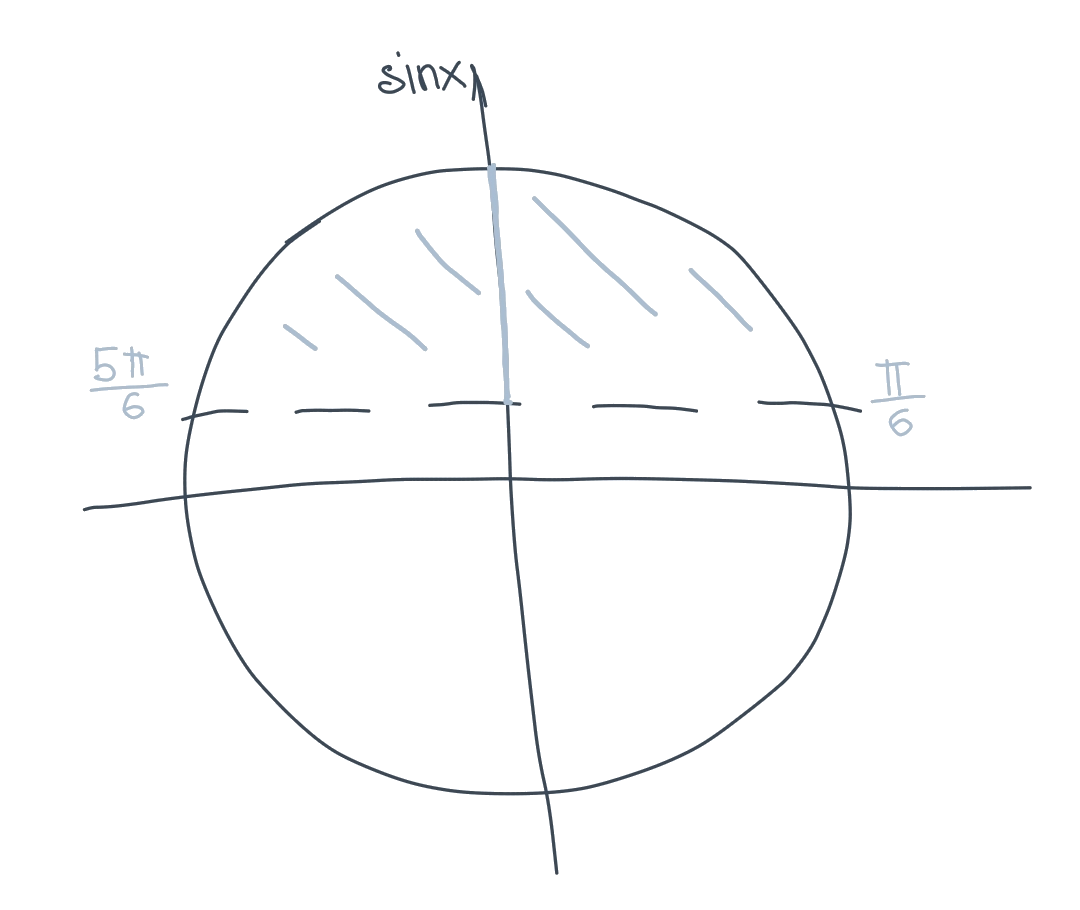
\includegraphics[scale=0.15]{sin_trigonometry}
        \end{figure}
    \end{enumerate}
\end{example}
%END TICKET 24